\begin{table*}[htbp]
    \centering
    \caption{Accuracy comparison across benchmarks and baselines. \toolname\ reports Pass@5 (cf.\ Table~\ref{tab:performance_rates_model}); baselines use their best reported configuration.}
    \label{tab:comparison}
    \begin{adjustbox}{max width=\linewidth}
    \begin{tabular}{l cccccccc}
        \toprule
        \textbf{Method} & \textbf{SyGuS} & \textbf{OOPSLA} & \textbf{SV-COMP} & \textbf{NLA} & \textbf{numer-S}  & \textbf{Frama-C} & \textbf{pIp} & \textbf{list-S}\\
        \midrule
        CODE2INV & 54.9\% & --- & --- & --- & ---& ---& ---& ---\\
        HOLA   & ---  & \textbf{93.5\%} & --- & --- & 
        --- & ---& ---& ---
        \\
        CLN2INV  & 93.2\% & --- & ---& --- &  --- & ---& ---& ---\\
        LIPuS & 93.2\% & --- & --- & 83.3\% & --- &  --- & ---& ---\\
         CLAUSE2INV & 99.2\% & --- & ---& \textbf{93.3\%} &  --- & ---& ---& --- \\
        \midrule
        \autospec-3.5  & 85.7\% & 82.6\% & \textbf{76.2\%}& {\cellcolor{gray!15}70.0\% }& {\cellcolor{gray!15}75.0\% } & 60.8\% & {\cellcolor{gray!15}14.0\% } & {\cellcolor{gray!15}0.0\% }\\
        \autospec-4o  & {\cellcolor{gray!15}86.5\%} &  {\cellcolor{gray!15}71.7\%} & {\cellcolor{gray!15}66.7\%}& {\cellcolor{gray!15}70.0\% }& {\cellcolor{gray!15}72.5\% } & {\cellcolor{gray!15}68.6\% }& {\cellcolor{gray!15}22.0\% } & {\cellcolor{gray!15}0.0\% }\\
        \autospec-Claude 3.7  & {\cellcolor{gray!15}88.7\%} &  {\cellcolor{gray!15}80.4\%} & {\cellcolor{gray!15}66.7\%}& {\cellcolor{gray!15}60.0\% }& {\cellcolor{gray!15}55.0\% } & {\cellcolor{gray!15}74.5\% }& {\cellcolor{gray!15}4.0\% } & {\cellcolor{gray!15}0.0\% }\\
        ACInv-3.5 & 71.4\% & 45.7\% & 42.9\% & --- & ---  & 34.5\% & ---  & --- \\
        ACInv-4o  & 79.9\% & 76.1\% & \textbf{76.2\%} & --- & ---  & 48.3\% & ---  & --- \\
        \toolname-3.5 & 93.2\% & 52.2\% & 66.7\% & 56.7\% &67.5\% & 51.0\% & 76.0\% & 16.7\%\\
        \toolname-4o     & 99.2\% & 76.1\% & \textbf{76.2\%} & 86.7\% & 82.5\% & 72.6\% & 78.0\% & 79.2\% \\
            \toolname-Claude 3.7 & \textbf{100.0\%} & 87.0\% & \textbf{76.2\%} &  86.7\% &  \textbf{85.0}\% & \textbf{76.5}\% & \textbf{88.0}\% & \textbf{95.8}\%
        \\
        \bottomrule
    \end{tabular}
    \end{adjustbox}
\end{table*}


\smallskip
\noindent\textbf{Overall comparison with LLM-based approaches.}
Table~\ref{tab:comparison} compares \autospec, ACInv, and \toolname; \specgen\ is omitted here because it targets Java/JML rather than C/ACSL. On the four datasets originally introduced by \autospec, \toolname\ achieves higher accuracy than ACInv on both GPT-3.5-turbo and GPT-4o, and both tools show similar gains from upgrading the model.

In contrast, \autospec\ barely improves from GPT-3.5-turbo to GPT-4o. Its reliance on few-shot prompting plus exhaustive sampling and verification-based filtering caps the gain that stronger models can deliver, so our \autospec-4o reproduction stays close to the reported \autospec-3.5 numbers.

\toolname\ instead gains steadily with stronger models. Its workflow requires complex reasoning --- program-execution simulation plus verifier-guided invariant refinement --- which exceeds GPT-3.5-turbo's instruction-following limits. Symbolic execution narrows this reasoning surface, so stronger models like GPT-4o benefit more.

The \textbf{pIp} fragments make this concrete: \autospec\ with Claude 3.7 Sonnet performs poorly despite Claude's strong reasoning, because Claude struggles to emit syntactically correct ACSL, and a specification that does not parse is never verified. \toolname\ avoids this with an ACSL skeleton built from the symbolic state, which both fixes the surface syntax and pins down the symbolic facts each clause must state; its advantage here is therefore semantic as well as syntactic.

\smallskip
\noindent\textbf{Detailed results across benchmarks.}
Against SMT-based numerical baselines, \toolname\ is on par with CLAUSE2INV on \textbf{SyGuS}, exceeds LIPuS on the nonlinear \textbf{NLA} benchmark while trailing CLAUSE2INV by 6.6\,pp, and achieves 87\% on the harder nested/multi-loop \textbf{OOPSLA} dataset. These SMT-based tools are specialized for numerical loops.

Against the LLM baselines \autospec\ and ACInv on numerical benchmarks, \toolname\ scores 15\% higher on \textbf{SyGuS} and higher on \textbf{NLA} and \textbf{numer-S}; on \textbf{OOPSLA} it matches ACInv and is only marginally below \autospec\ (with Claude 3.7 Sonnet, \toolname\ is 5\% higher). All three tools perform equally on \textbf{SV-COMP}, likely because the dataset is dominated by nested/multi-loop cases that no current approach solves. Overall, symbolic guidance captures specification facts that pure neural baselines miss on these benchmarks.

On \textbf{Frama-C}, \toolname\ improves over \autospec\ via inductive-predicate support, which enables more expressive specifications. On the industrial \textbf{pIp} fragments (structs and pointer operations), the flattened memory model plus symbolic execution gives an average 50\% higher success rate than \autospec. On the linked-list \textbf{list-S} benchmark, \toolname\ also performs well; \autospec\ cannot handle this class because it lacks inductive-data-type support.


\begin{finding}
\textbf{Finding (RQ4).} \toolname\ matches tools specialized for numerical invariants and clearly outperforms LLM-based generators (\autospec, ACInv), with the largest margins on the pointer-, struct-, and linked-list families that prior LLM tools handle poorly; its accuracy also scales with model capability where \autospec's plateaus.
\end{finding}






% --- Goal-masking experiment commented out (basis/data to be revisited) ---
% \begin{figure}[htbp]
%     \centering
%     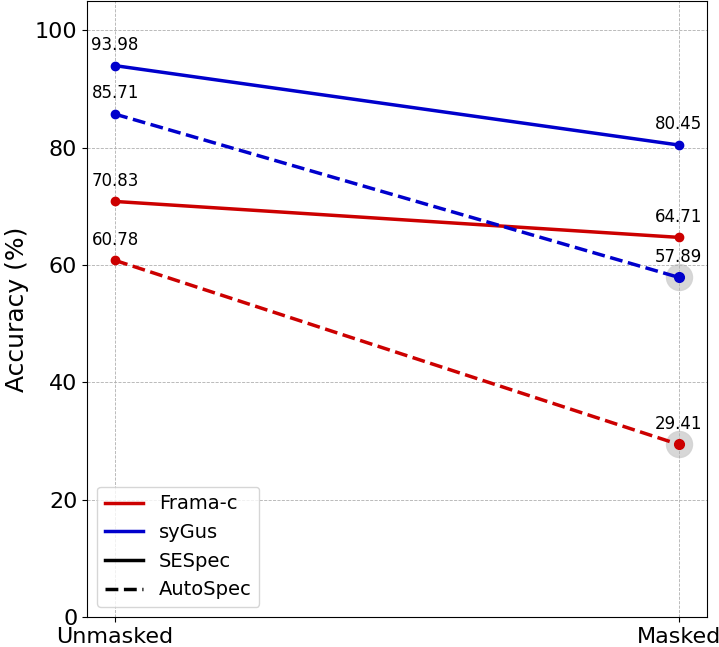
\includegraphics[width=0.95\linewidth]{images/mask.png}
%     \caption{Impact of masking verification goals. Gray-shaded dots are results we reproduced for AutoSpec.}
%     \label{fig:mask}
% \end{figure}
%
% \smallskip
% \noindent\textbf{Specification generation without verification goals.}
% As a final comparison axis, we measure how robustly each tool retains accuracy when the verification goal is removed --- the goal-independent setting that motivates \toolname. We evaluate this on \textbf{SyGuS} and \textbf{Frama-C} by masking the verification goals, running GPT-4o Pass@1 for \toolname\ and AutoSpec's reported configuration~\cite{autospec}.
% As shown in Fig.~\ref{fig:mask}, \toolname's accuracy drops modestly --- 93.98\%$\to$80.45\% on SyGuS and 70.83\%$\to$64.71\% on Frama-C --- while AutoSpec drops much more: 85.71\%$\to$57.89\% on SyGuS, 60.78\%$\to$29.41\% on Frama-C.
%
% The remaining drop of \toolname\ comes from the loss of assertion-failure feedback during refinement. In the unmasked setting, a failed assertion obligation tells the refinement loop which invariant or specification needs to be strengthened for the target proof. Once the assertion is masked, this target-specific strengthening signal is unavailable; when refinement is disabled, the masked and unmasked settings are nearly identical, indicating that the initial symbolic-state-guided generation is largely independent of the explicit assertion text.
